%----------------------------------------------------------------------------------------
%	CHAPTER 3
%----------------------------------------------------------------------------------------

\chapterimage{pano-tv1.png} % Chapter heading image
\acresetall

\cleardoublepage

\lgf{\chapter{ARCHITECTURE DE L'INTERNET}}
\lge{\chapter{ARCHITECTURE OF THE INTERNET}}

\lgf{\section{Les protocoles}}
\lge{\section{Protocols}}
  
    \vspace{1em}

  \begin{wrapfigure}{r}{8.5cm}
\centerline{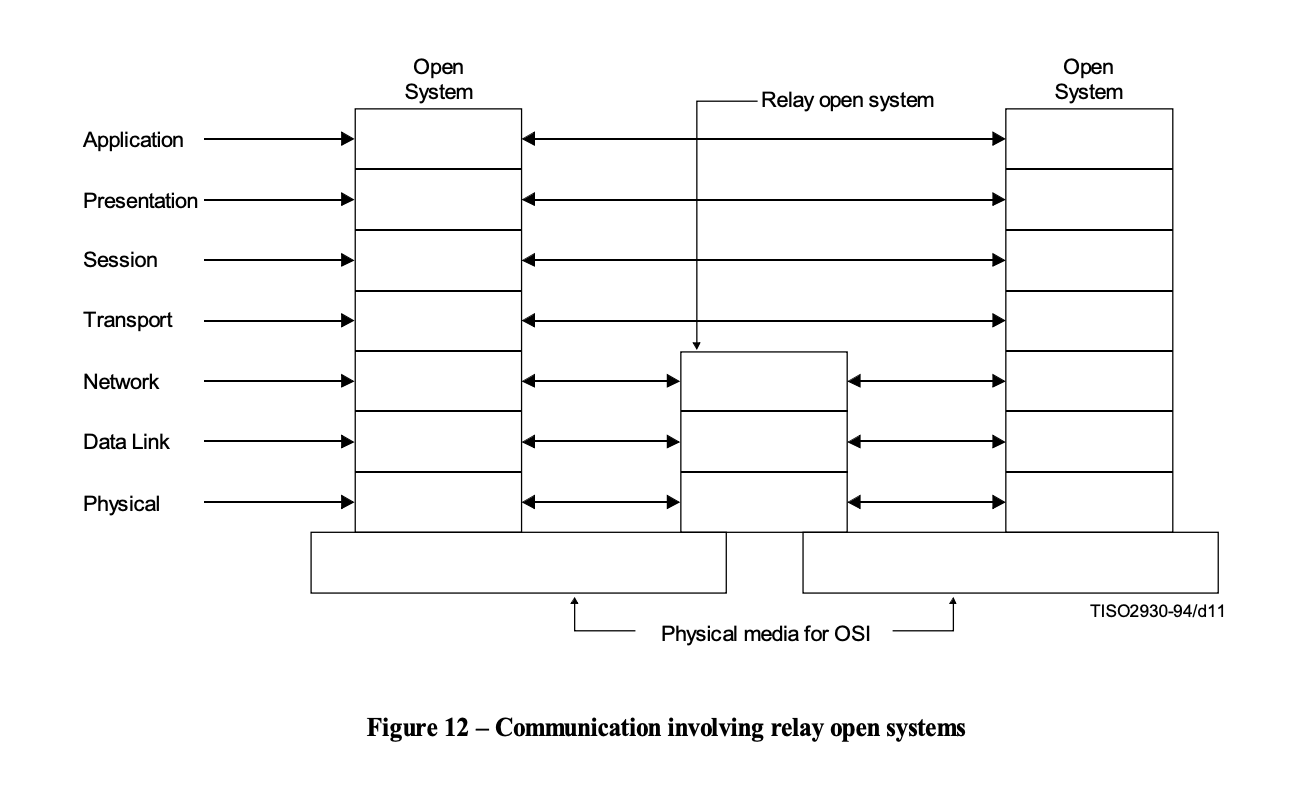
\includegraphics[width=.6\columnwidth]{Pictures/OSI.png}}
\lgf{\caption{Extrait du standard ITU-T Rec. X.200 (1994 E)}}
\lge{\caption{Extract from ITU-T Rec. X.200 (1994 E)}}
\end{wrapfigure}

\lgf{Vous connaissez sûrement le principe d'empilement protocolaire dans les réseaux. Chaque protocole fournit un service et se base sur celui de la couche inférieure pour le réaliser. Le modèle d'origine définit sept couches pour transporter les données d'une application, n'importe où dans le monde.
Les protocoles réseaux sont empilés les uns sur les autres, ceux du dessus utilisent les services offerts par ceux d’en dessous pour acheminer la donnée. Cela a donné lieu au modèle de référence de l’\ac{ISO} qui structure les réseaux depuis les années 1970. En théorie, il y a 7 \Index{couche}s, mais l'internet a fait évoluer ce modèle et les numéros des couches, associés à des fonctionnalités, sont restés~; ce qui peut conduire à une numérotation étrange.}
\lge{You probably know the principle of protocol stacking in networks. Each protocol provides a service and relies on the lower layer to perform it. The original model defines seven layers to transport the data of an application, anywhere in the world.
The network protocols are stacked on top of each other, with those above using the services offered by those below to carry the data. This gave rise to the reference model of the \ac{ISO} which has been structuring networks since the 1970s. In theory, there are 7 \Index{layer}s, but the Internet has made this model evolve and the numbers of the layers, associated with functionalities, have remained; this can lead to a strange numbering.}  
  
 \begin{figure}[tbp]
\centerline{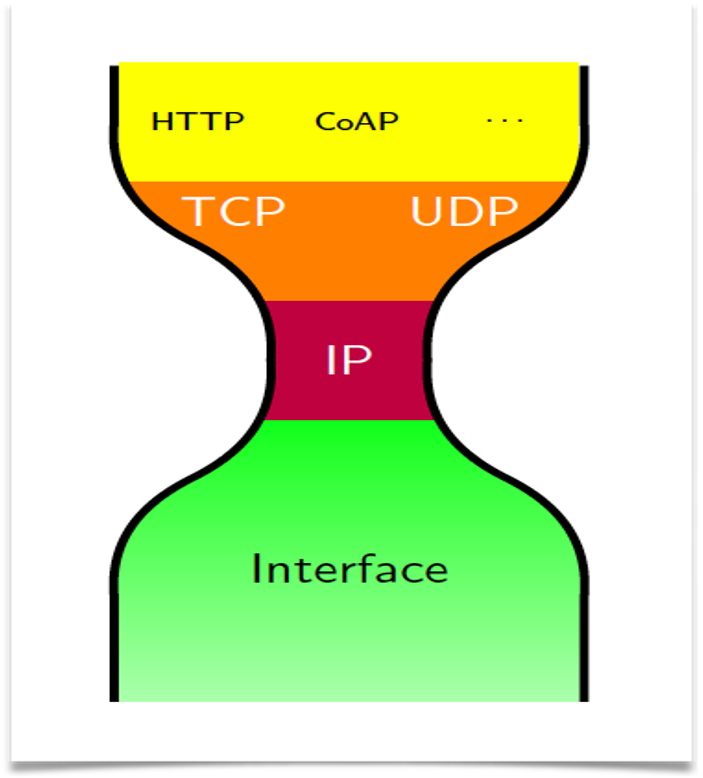
\includegraphics[width=.5\columnwidth]{Pictures/hourglass.png}}
\lgf{\caption{Empilement protocolaire de l'Internet}}
\lge{\caption{Protocol layering of the Internet}}
\label{fig-hourglass}
\end{figure}

  \vspace{1em}

\begin{wrapfigure}{r}{3cm}
\Youtube{https://youtu.be/vQ7zMVrqHbA}
\end{wrapfigure}

\lgf{L'internet a simplifié cette architecture (cf. figure~\vref{fig-hourglass}). C'est pour ça que l'on retrouve moins de couches et que les numéros ne sont pas contigus. }
\lge{The Internet has simplified this architecture (see figure~\vref{fig-hourglass}). That's why there are fewer layers and the numbers are not contiguous. }
  
  
    \vspace{1em}

\lgf{Les deux premières couches  en partant du bas, regroupées sous le nom d'Interface, permettent de transmettre les données binaires sur un support physique. La couche 1 s’occupe de cette modulation sur un support physique particulier (fibre optique, paire de cuivre, onde radio). La couche 2 regroupe les mécanismes qui permettent de structurer cette donnée sous forme de bloc de taille finie appelées trames, de définir les méthodes d’accès, c’est-à-dire quand l’équipement peut émettre, et les formats des adresses utilisées pour identifier les équipements.}
\lge{The first two layers from the bottom, grouped under the name of Interface, allow the transmission of binary data on a physical medium. Layer 1 deals with this modulation on a particular physical medium (optical fiber, copper pair, radio wave). Layer 2 groups together the mechanisms that allow this data to be structured in finite size blocks called frames, to define the access methods, i.e. when the equipment can transmit, and the address formats used to identify the equipment. }


\begin{itemize}
\item 
    \lgf{l’\ac{IEEE} qui propose des standards comme Ethernet pour les réseaux filaires ou Bluetooth et Wifi pour les réseaux radio,}
    \lge{the \ac{IEEE} which proposes standards like Ethernet for the wired networks or Bluetooth and Wifi for the radio networks,}
    
\item 
    \lgf{le \ac{3GPP}  qui opère au même niveau et définit les protocoles pour la téléphonie cellulaire (4G),}
    \lge{the \ac{3GPP} which operates at the same level and defines the protocols for cellular telephony (4G),}
    
\item \ldots
\end{itemize}

  
    \vspace{1em}

  
  
\lgf{Au-dessus, on a le protocole \ac{IP} standardisé par l'IETF.  Le protocole \ac{IP} s’adapte simplement à tout moyen de communication. \ac{IP} propose ainsi une abstraction des moyens de communication aux couches applicatives, rendant l’accès au réseau et l’adressage universels. Le traitement dans les \Index{routeur}s (équipements chargés d’aiguiller l’information dans le réseau) doit être le plus rapide possible pour traiter un maximum de paquets par seconde. De plus, \ac{IP} ne spécialise pas le réseau pour un service ou un autre ; il ne fait qu’aiguiller les paquets vers la bonne destination. Le réseau Internet est un réseau mondial construit autour de ce protocole permettant potentiellement d'atteindre tous les équipements qui y sont connectés. }
\lge{Above, we have the IETF standardized protocol.  The \ac{IP} protocol adapts simply to any medium of communication. \ac{IP} thus proposes an abstraction of the means of communication for the application layers, making the access to the network and the addressing universal. The treatment in the \Index{router}s (equipment in charge of routing the information in the network) must be as fast as possible to treat a maximum of packets per second. Moreover, \ac{IP} does not specialize for one service or another; it only routes the packets to the right destination. The Internet is a worldwide network built around this protocol, potentially reaching all the equipment connected to it. }

  
  
\lgf{Les experts de l'internet aiment cette représentation en \Index{sablier} où \ac{IP} apparaît en position centrale mais est plus petit comparé aux autres protocoles. Par conception, \ac{IP} est très simple ; à la fois pour être portés facilement sur de nombreux niveaux 2 et être facilement utilisable par les couches hautes, mais également pour traiter les données très rapidement dans les nœuds d'interconnexion.}
\lge{Internet experts like this representation in \Index{hourglass} where \ac{IP} appears in a central position but is smaller compared to the other protocols. By design, IP is very simple; both to be easily ported to many Layer 2s and to be easily used by higher layers, but also to process data very quickly in the interconnection nodes.}

  
\lgf{\ac{IP} est mis en oeuvre partout sur Internet aussi bien dans les équipements en extrémité du réseau que dans les routeurs chargés d'envoyer les données vers la bonne destination.}
\lge{\ac{IP} is implemented everywhere on the Internet as well in the equipment at the end of the network as in the routers in charge of sending the data to the right destination.}

    \vspace{1em}

\lgf{Au-dessus on trouve deux protocoles qui ne sont mis en oeuvre que dans les équipements d'extrémité.  Si le niveau 3 permet de joindre une machine, le niveau 4 va permettre d’identifier l'application qui doit traiter les données. Les "adresses" de ces applications sont des numéros compris entre 1 et 65535 appelés \Index{port}s. Par exemple, les serveurs Web utilisent le port numéro 80 ou le numéro 443. }
\lge{Above that are two protocols that are only implemented in the end devices.  If level 3 allows to reach a machine, level 4 will allow to identify the application which must process the data. The "addresses" of these applications are numbers between 1 and 65535 called \Index{port}s. For example, Web servers use port number 80 or 443. }

\lgf{Le protocole \ac{TCP} va surveiller les données transférées et sera capable de retransmettre des données perdues, ralentir ou accélérer le transfert de données s’il détecte une saturation du réseau. En revanche, sa mise en œuvre est complexe et coûteuse en mémoire. Dans les cas simple, \ac{UDP} est préféré ; il n'apporte pas de traitement supplémentaire \ac{UDP}, c'est un protocole minimal qui se contentent d'aiguiller les données vers la bonne application sans aucun autre contrôle.}
\lge{The protocol \ac{TCP} will monitor the transferred data and will be able to retransmit lost data, slow down or accelerate the data transfer if it detects a network saturation. On the other hand, its implementation is complex and costly in memory. In the simple cases, \ac{UDP} is preferred; it does not bring additional treatment \ac{UDP}, it is a minimal protocol which is satisfied to direct the data towards the good application without any other control.}

  

    \vspace{1em}

  
\lgf{Au-dessus, on trouve les applications qu'historiquement on classe dans la couche 7. Les applications sont très nombreuses mais la plus répandue est \ac{HTTP} qui sert à transporter les pages web, mais également elle permet des communications directes entre ordinateurs. }
\lge{Above, we find the applications that historically are classified in layer 7. The applications are very numerous but the most widespread is \ac{HTTP} which is used to transport the Web pages, but also it allows direct communications between computers. }

  
  
    \vspace{1em}


   \begin{figure}[tbp]
\centerline{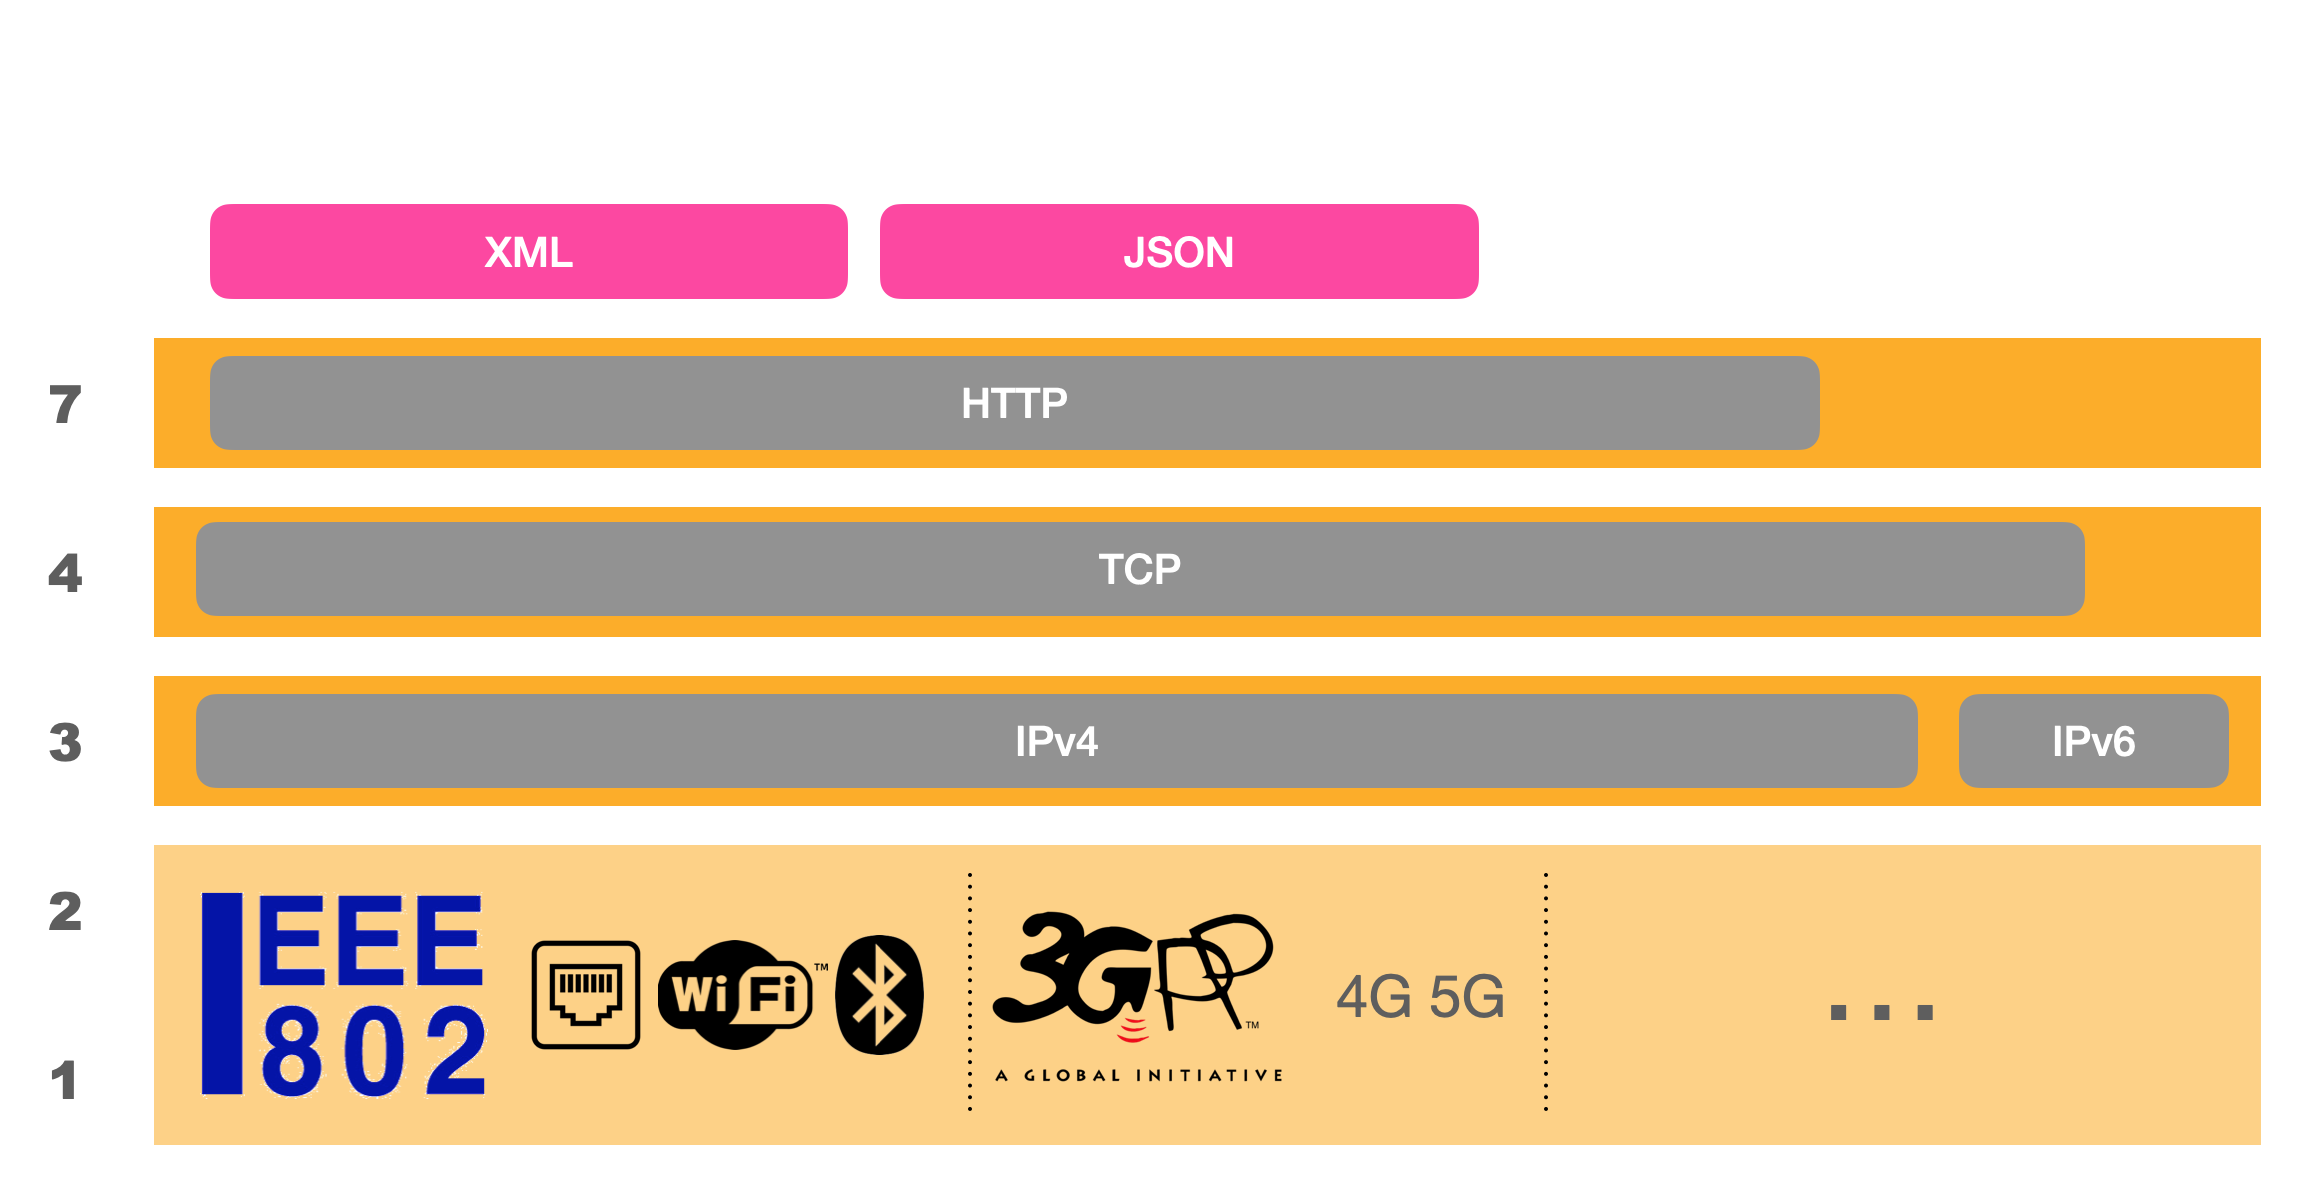
\includegraphics[width=1\columnwidth]{Pictures/fullIPstack.png}}
\lgf{\caption{Principaux protocoles de l'Internet}}
\lge{\caption{Main Internet protocols}}
\label{fig-fullstack}
\end{figure}

\lgf{Pour le grand public, l’internet désigne surtout la totalité de cet assemblage protocolaire et est souvent confondu avec l’application qui a démocratisé son usage : le Web.  C'est vrai également pour les techniciens, le trafic produit par le Web est largement présent dans l'Internet. Ce schéma, figure~\vref{fig-fullstack} reprend la pile protocolaire majoritairement utilisé dans l'internet. On voit qu'au niveau 3 on a deux versions du protocole \ac{IP} ; la version 4 est la version historiquement déployée et elle a eu tellement de succès qui est de plus en plus difficile d'avoir des adresses \ac{IPv4} pour les machines. Pour permettre au réseau de continuer de fonctionner, une nouvelle version a été développée. \ac{IPv6} rend l'adressage quasi infini avec des adresses sur 128 bits. \ac{IPv6} gagne petit à petit du terrain dans les usages classiques et c'est surtout une brique essentielle pour l'internet des objets. }
\lge{For the general public, the Internet designates above all the totality of this protocol assembly and is often confused with the application that democratized its use: the Web.  This is also true for technicians, the traffic produced by the Web is largely present in the Internet. This diagram, figure~\vref{fig-fullstack} shows the protocol stack that is mostly used in the Internet. We see that at level 3 we have two versions of the protocol; version 4 is the version historically deployed and it has been so successful that it is more and more difficult to have addresses for machines. To keep the network running, a new version has been developed. \ac{IPv6} makes the addressing almost infinite with addresses on 128 bits. \ac{IPv6} gains little by little ground in the traditional uses and it is especially an essential brick for the Internet of the objects. }
  
\lgf{Le Web utilise majoritairement le protocole \ac{HTTP}. Et comme \ac{HTTP} repose sur \ac{TCP}, ces deux protocoles sont dominants sur le réseau. }
\lge{The Web uses mainly the protocol \ac{HTTP}. And as \ac{HTTP} relies on \ac{TCP}, these two protocols are dominant on the network. }
  
\lgf{Finalement ce graphique ajoute une couche supplémentaire, au-dessus de la couche 7, pour indiquer comment les données transportées sont structurées avec des formats comme \ac{XML} ou \ac{JSON} que nous verrons dans la suite.}
\lge{Finally this graph adds an additional layer, above layer 7, to indicate how the transported data is structured with formats like \ac{XML} or \ac{JSON} that we will see in the following.}

  
  
  \Question{\lgf{Pile Protocolaire}\lge{Protocol Stack}}
  {\lgf{Dans la pile protocolaire de l'internet, quels protocoles ont pour fonction d'aiguiller les paquets jusqu'à leur destination (2 réponses) }
   \lge{In the internet protocol stack, which protocols are responsible for routing packets to their destination (2 answers) }  
  \begin{multicols}{4}
  \begin{itemize}[label=$\square$]
   \item \Wrong{Ethernet}
   \item \Wrong{IEEE}
   \item \Wrong{802.15.5}
   \item \Wrong{Wi-Fi}
   \item \Correct{IPv4}
   \item \Correct{IPv6}
   \item \Wrong{UDP}
   \item \Wrong{TCP}
   \item \Wrong{MQTT} 
   \item \Wrong{HTTP}
   \item \Wrong{CoAP}
   \item \Wrong{XML}
   \item \Wrong{JSON}
  \end{itemize}
  \end{multicols}
  }
  {
  \lgf{Le protocole \ac{IP} permet de transporter l'information d'un bout à l'autre du réseau en utilisant les adresses \ac{IP} contenues dans les paquets. Il existe deux versions de ce protocole \ac{IPv4} initialement déployé et \ac{IPv6} qui offre beaucoup plus de capacité d'adressage.}
  \lge{The protocol \ac{IP} makes it possible to transport information from one end of the network to the other by using the addresses \ac{IP} contained in the packets. There are two versions of this protocol : \ac{IPv4} initially deployed and \ac{IPv6} which offers much more addressing capacity.}
  }
  
\lgf{\section{Les fondements du Web}}
\lge{\section{Foundations of the Web}}

  
    \vspace{1em}
\begin{wrapfigure}{r}{3cm}
\Youtube{https://youtu.be/PKKzV-Vy33s}
\end{wrapfigure}

\lgf{L'architecture qui a conduit au Web est une formidable source d’inspiration pour le développement de nouveaux services car il est l’un des plus grands succès reposant sur le réseau Internet. Le Web forme de grands systèmes distribués et repose sur plusieurs principes qui le rendent universel et évolutif. La navigation avec un navigateur n’est que la partie visible du trafic ; les principes du web sont également utilisés pour le streaming vidéo, les échanges entre ordinateurs.}
\lge{One of the most important success stories based on the Internet is the architecture that led to the Web since it is a great source of inspiration for the development of new services. The Web forms large distributed systems and is based on several principles that make it universal and scalable. Surfing with a browser is only the visible part of the traffic; the principles of the web are also used for video streaming, exchanges between computers.}

  
\lgf{Le Web et ses extensions sont basés sur un modèle client-serveur. Les serveurs possèdent des ressources et les clients peuvent y accéder ou les modifier grâce à un protocole tel que \ac{HTTP}. Le modèle client-serveur est quelque chose de courant dans les réseaux informatiques, mais le Web suit certaines directives de conception connues sous le nom de \ac{REST}.}
\lge{The Web and its extensions are based on a client-server model. Servers own resources and clients can access or modify them through a protocol such as \ac{HTTP}. The client-server model is something common in computer networks, but the Web follows certain design guidelines known as \ac{REST}.}


    \vspace{1em}

\lgf{Selon Roy Fielding, qui a défini ce modèle~\cite{rest}, \ac{REST} est un ensemble de principes, de propriétés et de contraintes. \ac{REST} utilise le modèle de communication client-serveur et utilise généralement le protocole \ac{HTTP}.}
\lge{According to Roy Fielding, who defined this model, \ac{REST} is a set of principles, properties and constraints. \ac{REST} uses the client-server communication model and generally uses the \ac{HTTP} protocol.}

\lgf{Le principe \ac{REST} permet de concevoir des serveurs évolutifs. Un serveur doit être sans état, ce qui signifie qu’il ne conserve pas d’information après avoir répondu à une demande d’un client. Cela permet de simplifier le traitement dans le serveur qui doit traiter les requêtes d'un grand nombre de clients. }
\lge{The \ac{REST} principle allows to design scalable servers. A server must be stateless, which means that it does not retain any information after responding to a client request. This simplifies the processing in the server that has to handle requests from a large number of clients. }


\lgf{Cela impose que l’état soit situé du côté du client. Cet état est alimenté à partir des données structurées que le client reçoit du serveur. Ainsi, lorsqu’un client demande une page Web, celle-ci peut contenir d’autres \ac{URI} pour la compléter, par exemple des images, des feuilles de style, des scripts, etc.}
\lge{This requires that the report be located on the client side. This state is fed from the structured data that the client receives from the server. Thus, when a client requests a Web page, it can contain other \ac{URI} to complete it, for example images, style sheets, scripts, etc.}


\lgf{Le client doit donc comprendre les données que le serveur lui envoie et donc connaître le format de représentation de la ressource qu'il reçoit pour y retrouver les \ac{URI}. Donc, en plus de la ressource elle-même, le serveur ajoute des informations complémentaires, appelées métadonnées. Elles intègrent entre autres le format du contenu (content format). Il peut s’agir de texte pur, d’une image ou d’un format de texte structuré tel que \ac{HTML} ou \ac{JSON}.}
\lge{The client must therefore understand the data that the server sends him and therefore know the representation format of the resource that he receives in order to find the \ac{URI}. In addition to the resource itself, the server adds additional information, called metadata. Among other things, this information includes the format of the content (content format). It can be pure text, an image or a structured text format such as \ac{HTML} or \ac{JSON}.}
  
      \vspace{1em}

\lgf{\subsection{Ressources}}
\lge{\subsection{Resources}}

    \vspace{1em}

   \begin{wrapfigure}{r}{9cm}
\centerline{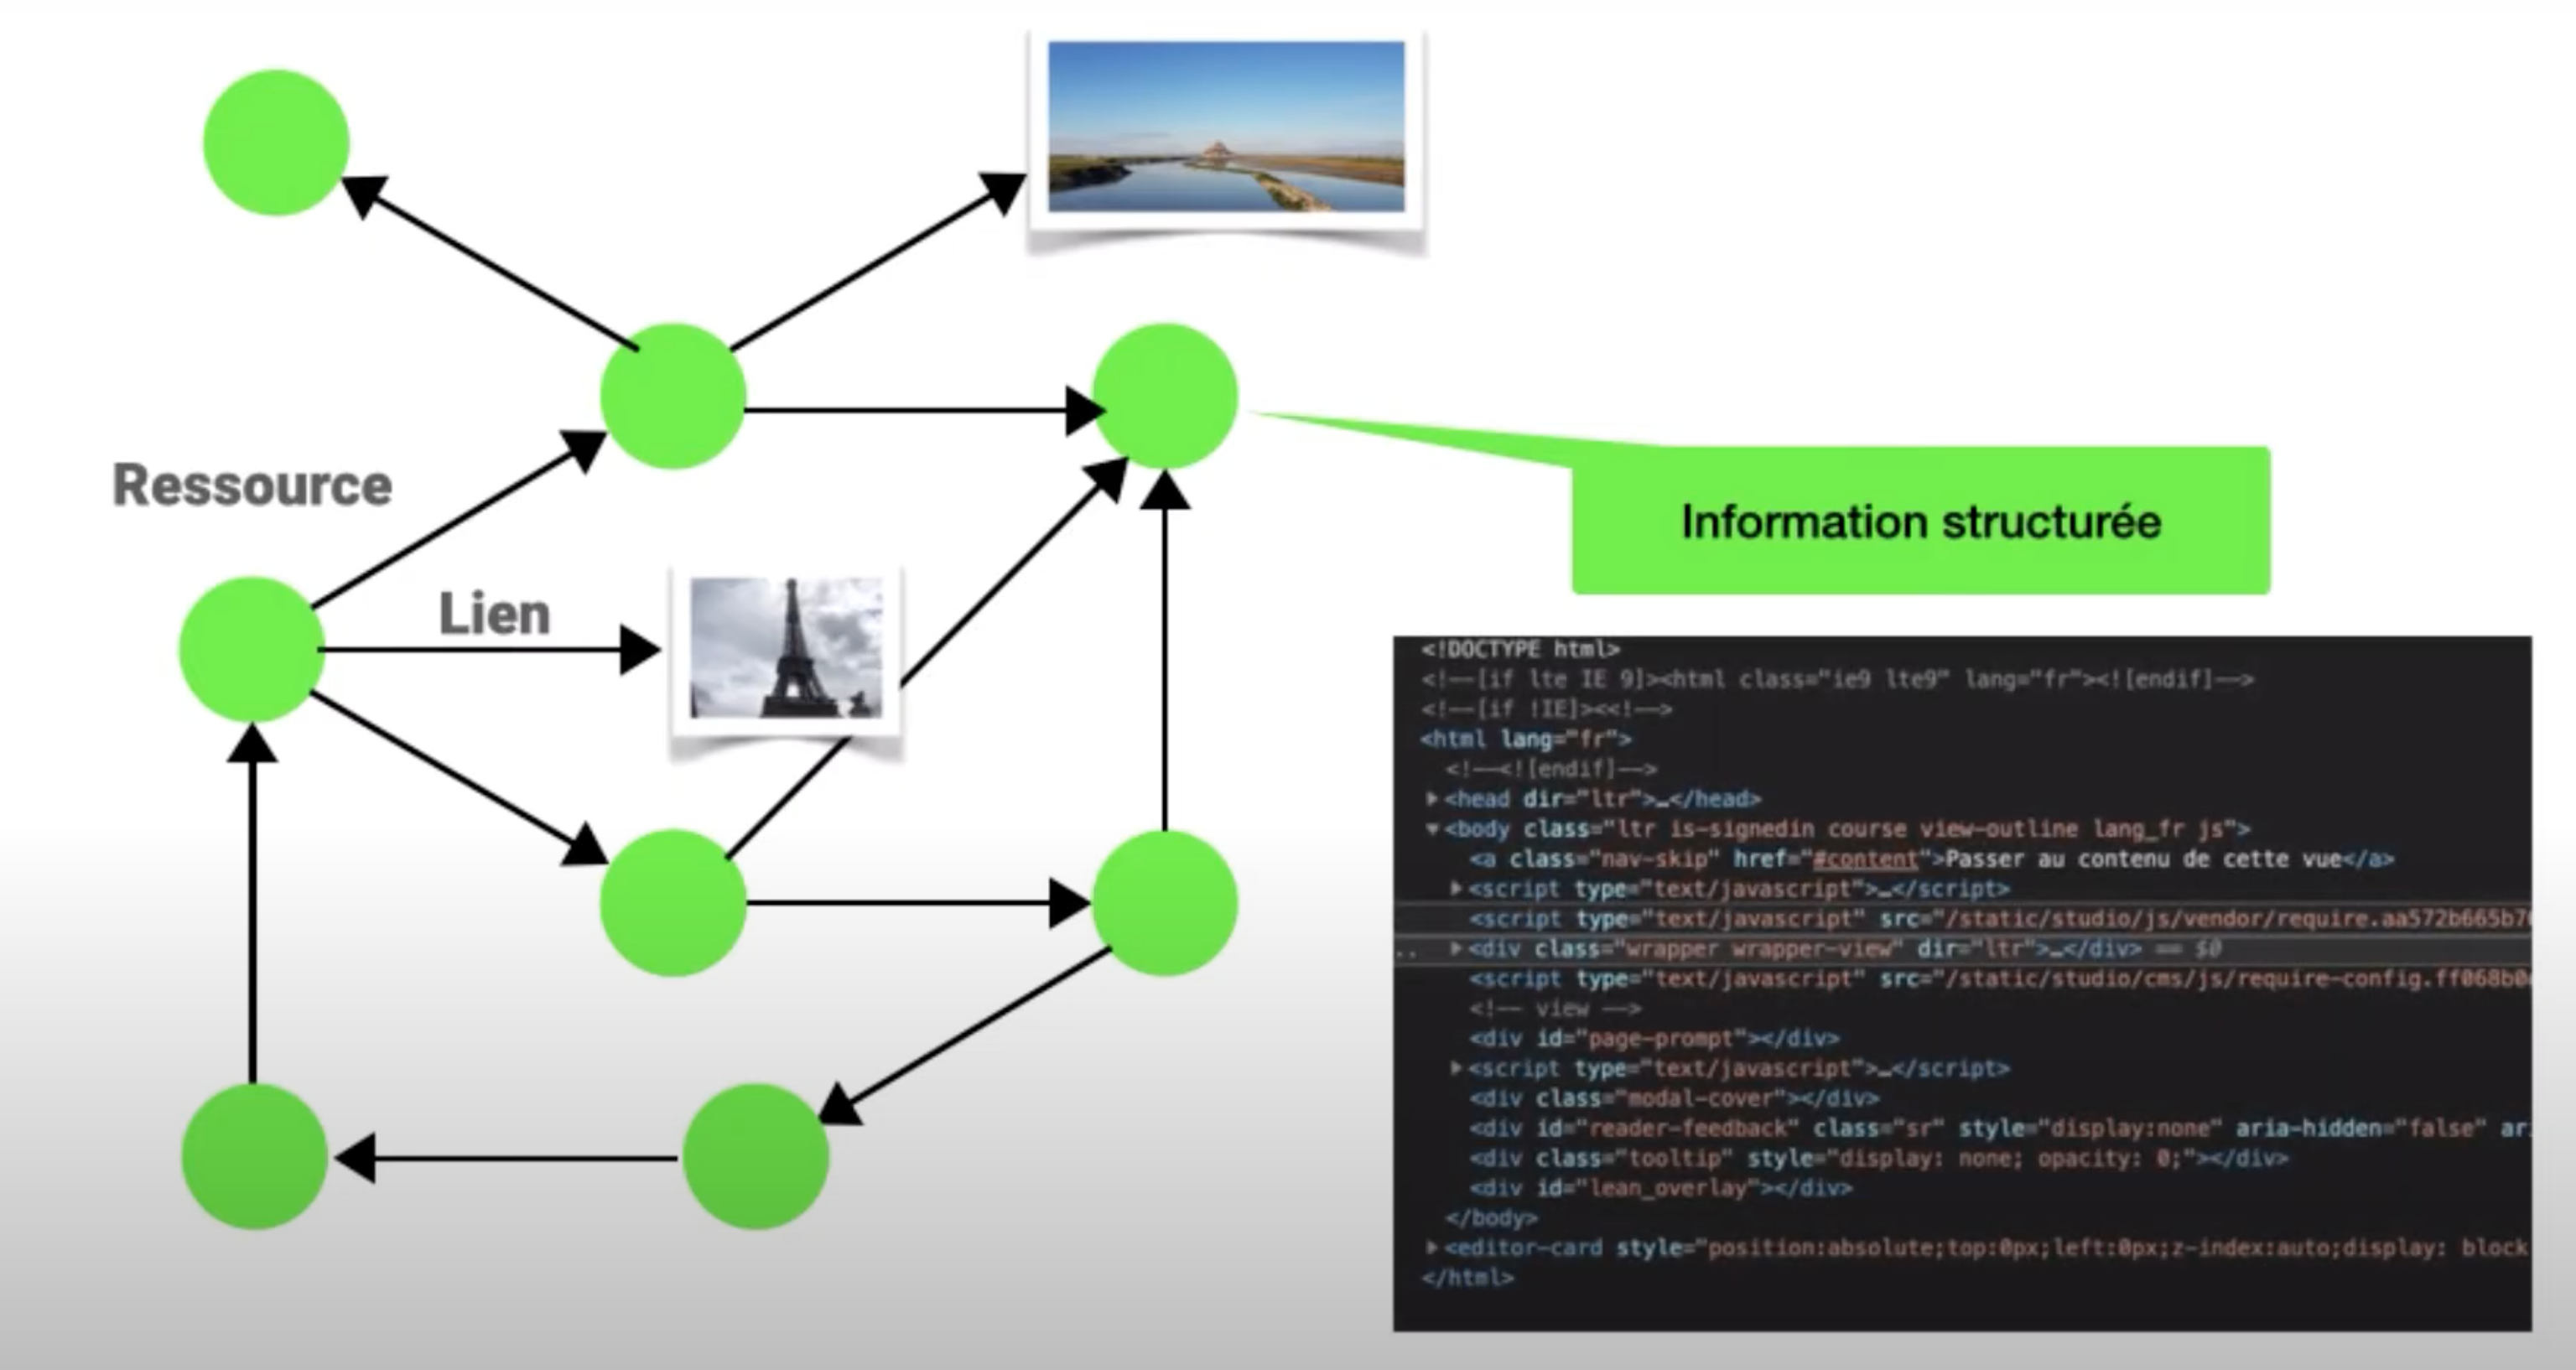
\includegraphics[width=.6\columnwidth]{web.png}}
\end{wrapfigure}


\lgf{L'élément de base est la ressource que l'on peut définir comme un bloc de données de taille finie. Les ressources peuvent elles-mêmes contenir des références à d'autres ressources qui à leur tour vont faire référence à d'autres ressources etc. Cela forme un maillage entre ressources qui est comparé à une toile d'araignée (web en anglais). La ressource peut être, par exemple, une image dans ce cas elle ne fera pas référence à autre chose. Pour faire référence à une autre ressource, son contenu doit être structuré et doit donc être défini dans un format où l'on peut facilement comprendre qu'une partie du contenu est une référence a une autre ressource. HTML est un de ces langages qui permet aux pages web de se référencer entre elles par le biais de liens. }
\lge{The basic element is the resource, which can be defined as a data block of finite size. Resources can themselves contain references to other resources which in turn will refer to other resources etc. This forms a mesh between resources which is compared to a spider's web. The resource can be, for example, an image in which case it will not refer to anything else. To refer to another resource, its content must be structured and therefore defined in a format where it is easy to understand that part of the content is a reference to another resource. HTML is one such language that allows web pages to reference each other through links. }


  
      \vspace{1em}

\lgf{\subsection{Identifiants}}
\lge{\subsection{Identifiers}}

    \vspace{1em}

   
\lgf{Chaque ressource du Web est identifiée par une valeur unique appelée \ac{URI}. Si l’URI contient des caractères internationaux, (comme les lettres accentuées, ...)   il est appelé \ac{IRI}.}
\lge{Each Web resource is identified by a unique value called \ac{URI}. If the URI contains international characters, (like accented letters, ...) it is called \ac{IRI}.}


\lgf{Les \ac{URI} permettent de désigner une ressource de manière non ambiguë, c'est-à-dire que l'on ne retrouvera pas le même \ac{URI} pour désigner deux ressources différentes.  Par construction, la structure de l’\ac{URI} est hiérarchique, ce qui permet de créer des identificateurs uniques de manière distribuée. Si vous voulez identifier une ressource, vous devez posséder une séquence unique : un numéro de téléphone, un numéro de sécurité sociale, un nom de domaine. En y ajoutant quelque chose d'unique pour nous, cela crée un identifiant globalement unique.}
\lgf{The \ac{URI} allow to designate a resource in an unambiguous way, i.e. one will not find the same \ac{URI} to designate two different resources.  By construction, the structure of the \ac{URI} is hierarchical, which allows unique identifiers to be created in a distributed fashion. If you want to identify a resource, you must have a unique sequence: a phone number, a social security number, a domain name. By adding something unique to us, it creates a globally unique identifier.}


\lgf{Par exemple, pour identifier une image, on peut la nommer}
\lge{For example, to identify an image, we can name it}

\begin{termc}[backgroundcolor=\color{palerod}, language=json, basicstyle=\ttfamily, escapechar=@]
image
\end{termc}

\noindent
\lgf{mais il y a peu de chance que ce nom soit unique, d'autres personnes sur Terre ont sûrement eu la même idée. En revanche, si je la fais précéder de mon numéro de téléphone}
\lge{but there is little chance that this name is unique, other people on Earth have surely had the same idea. On the other hand, if I preface it with my phone number}

\begin{termc}[backgroundcolor=\color{palerod}, language=json, basicstyle=\ttfamily, escapechar=@]
33667789078image
\end{termc}


\noindent
\lgf{sera unique si je ne nomme qu'une seule ressource "image". Un autre utilisateur sur le même principe pourra nommer sa ressource :}
\lge{will be unique if I name only one resource "image". Another user on the same principle can name his resource :}

\begin{termc}[backgroundcolor=\color{palerod}, language=json, basicstyle=\ttfamily, escapechar=@]
33667239018image
\end{termc}


\noindent
\lgf{sans ambiguïté possible. Cependant, comme le numéro de téléphone est unique dans l'espace des numéros de téléphone, d'autres numéros uniques pourraient entrer en conflit dans d'autres espaces de numérotation. }
\lge{without any possible ambiguity. However, because the phone number is unique in the phone number space, other unique numbers could conflict in other numbering spaces. }

\lgf{Pour éviter les conflits, il est intéressant de donner, au début l'espace de numérotation, par exemple~:}
\lge{To avoid conflicts, it is interesting to give the numbering space at the beginning, for example:}

\begin{termc}[backgroundcolor=\color{palerod}, language=json, basicstyle=\ttfamily, escapechar=@]
tel:33667789078image
\end{termc}

\noindent
\lgf{et}
\lge{and}

\begin{termc}[backgroundcolor=\color{palerod}, language=json, basicstyle=\ttfamily, escapechar=@]
ss:33667789078image
\end{termc}


\noindent
\lgf{les deux identifiants seront uniques, même si le hasard a fait que ce numéro de téléphone et ce numéro de sécurité sociale coïncident.}
\lge{the two identifiers will be unique, even if by chance this phone number and this social security number coincide.}

      \vspace{1em}


\lgf{Les \ac{URI} formalisent ce principe. Le \rfc{3986} explique comment ils peuvent être construits. Un URI commence par un schéma indiquant l’autorité de nommage, suivi d’une valeur d’autorité puis d’un chemin dans l’espace d’autorité. Des caractères comme les ":" ou les "/" sont utilisés pour améliorer la lisibilité de l'\ac{URI}.}
\lge{The \ac{URI} formalize this principle. The \rfc{3986} explains how they can be constructed. A URI starts with a scheme indicating the naming authority, followed by an authority value and then a path in the authority space. Characters such as ":" or "/" are used to improve the readability of the \ac{URI}.}

\lgf{Par exemple~:}
\lge{For instance:}

\begin{termc}[backgroundcolor=\color{palerod}, language=json, basicstyle=\ttfamily, escapechar=@]
mailto:mduerst@ifi.unizh.ch
ssh://utilisateur@example.com
ftp://ftp.is.co.za/rfc/rfc1808.txt
\end{termc}


      \vspace{1em}

\lgf{Ainsi, si je mets une ressource sur un site Web, celui-ci est identifié par un nom de domaine, par exemple \texttt{example.com}. Je suis propriétaire de ce nom. Je peux donc l’utiliser pour identifier de manière unique ma ressource. Si on reprend le principe de construction d’un URI, j’aurai :}
\lgf{So, if I put a resource on a Web site, it is identified by a domain name, for example \texttt{example.com}. I own this name. I can therefore use it to uniquely identify my resource. If we take the principle of construction of a URI, I will have :}

\begin{termc}[backgroundcolor=\color{palerod}, language=json, basicstyle=\ttfamily, escapechar=@]
http://example.com/ma_ressource
\end{termc}

\lgf{Personne d’autre dans l’univers ne pourra identifier ses ressources avec cette chaîne de caractères puisque \texttt{example.com} m’appartient. Je dispose donc d’un espace de nommage infini qui me permet de désigner l’ensemble infini de ressources sans que personne d’autre ne puisse prendre les mêmes noms. Un \ac{URI} est une construction administrative permettant d’attribuer un identifiant unique global à une ressource spécifique.}
\lge{No one else in the universe will be able to identify their resources with this string since \texttt{example.com} belongs to me. I therefore have an infinite namespace that allows me to designate the infinite set of resources without anyone else being able to take the same names. An \ac{URI} is an administrative construct that allows you to assign a globally unique identifier to a specific resource.}


  \begin{figure}[tbp]
\centerline{
\includegraphics[width=1\columnwidth]{Pictures/Capture15.png}}
\lgf{\caption{Structuration d'une URI}}
\lge{\caption{Structure of a URI}}
\label{fig-stucURI}
\end{figure}

\lgf{L’\ac{URI} (cf.figure~\vref{fig-stucURI}) a pour but de facilement nommer une ressource, de pouvoir lier les ressources entre elles pour former cette toile d’araignée mondiale. Le schéma définit à la fois l'espace de nommage de l'autorité et son format. Une adresse \ac{IP} ou un nom de domaine comme autorité est à la fois un moyen d'assurer l'unicité globale, mais également de savoir comment accéder à la ressource. }
\lge{The \ac{URI} (cf.figure~\vref{fig-stucURI}) is intended to easily name a resource, to be able to link resources together to form this global spider web. The schema defines both the namespace of the authority and its format. An address or domain name as an authority is both a way to ensure global uniqueness, but also to know how to access the resource. }

      \vspace{1em}

\lgf{Par exemple, \Index{spotify} a défini son propre schéma et ensuite il n'a plus besoin d'autorité mais structure le chemin pour référencer une playlist. }
\lge{For example, \Index{spotify} has defined its own schema and then it no longer needs authority but structures the path to reference a playlist. }

\lgf{Tous les livres ont un numéro \ac{ISBN} qui permet d'identifier. Il peut être intégré aussi dans une URI. Il faut voir que ces deux types d'identifiants permettent de référencer un objet unique mais rien qu'en le lisant on ne peut pas accéder à la ressource. On appelle cette sous famille des \ac{URI}, des \ac{URN}.}
\lge{All the books have a number \ac{ISBN} which allows to identify. It can also be integrated in a URI. These two types of identifiers make it possible to refer to a single object but only by reading it one cannot reach the resource. This sub-family of \ac{URI} identifiers is called \ac{URN}.}

\lgf{Un sous-ensemble d’\ac{URI} peut être directement utilisé pour localiser la ressource, c’est-à-dire trouver sur quel serveur se trouve la ressource et comment y accéder. Il s’agit d’une \ac{URL} bien connue du grand public et utilisée par les navigateurs Web.}
\lge{A subset of \ac{URI} can be used directly to locate the resource, i.e. find out on which server the resource is located and how to access it. This is a \ac{URL} that is well known to the general public and used by Web browsers.}


\lgf{Le schéma http est bien pratique car il peut se lire également comme un \ac{URL}. Ce schéma donne~:}
\lge{The http schema is very convenient because it can also be read as an \ac{URL}. This scheme gives~:}

\begin{itemize}
\item 
    \lgf{le protocole à utiliser pour accéder à la ressource (http),}
    \lge{le protocole à utiliser pour accéder à la ressource (http),}
\item 
    \lgf{l’autorité qui indique l’adresse du serveur (et son port),}
    \lge{the authority that indicates the server address (and its port),}
\item 
    \lgf{et enfin, le chemin d’accès de ce que l'on va demander au serveur et qui peut parfois correspondre à une arborescence de fichiers sur un serveur.}
    \lge{and finally, the access path of what we are going to ask to the server and which can sometimes correspond to a tree of files on a server.}
\end{itemize}
   
   
       \vspace{1em}

\lgf{Mais il faut bien voir que le but initial est de faire un identifiant unique. Le schéma https donne la manière dont sera construit la suite et dans un second temps uniquement sera vu comme le protocole à utiliser pour accéder à la ressource. L'autorité est unique et dans un second temps servira à localiser le serveur. Et finalement le chemin va indiquer comment parvenir à accéder à la ressource sur le serveur. Donc les ressources de notre toile d'araignée mondiale sont présentes sur des serveurs et chaque ressource possède un identifiant unique. Dans un premier temps, le client connaît l'\ac{URI} d'une ressource. Si c'est une \ac{URL}, il peut contacter le serveur. Le serveur lui retourne la ressource. Le client l'analyse et découvre les \ac{URI} qu'il contient. Il peut donc interroger le ou les autres serveurs pour reconstruire localement une partie de la toile nécessaires au traitement que le client veut effectuer.}
\lge{But we must see that the initial goal is to make a unique identifier. The https schema gives the way the suite will be built and in a second time only will be seen as the protocol to use to access the resource. The authority is unique and in a second time will be used to locate the server. And finally the path will indicate how to access the resource on the server. So the resources of our global spider web are present on servers and each resource has a unique identifier. First, the client knows the \ac{URI} of a resource. If it is a URL, he can contact the server. The server returns the resource to him. The client analyses it and discovers the \ac{URL}s it contains. It can then question the other server(s) to reconstruct locally a part of the web necessary for the treatment that the client wants to carry out.}

  
         \vspace{2em}

\Question{\lgf{Unicité}\lge{Unicity}}
{
\lgf{Qu'est ce qui est unique dans le monde (6 réponses) ?}
\lge{What is unique in the world (6 answers)?}
\begin{itemize}[label=$\square$]
\item \Wrong{
    \lgf{Un prénom.}
    \lge{A first name.}
    }
\item \Wrong{
    \lgf{Un nom de famille.}
    \lge{A family name.}
    }
\item \Correct{
    \lgf{un numéro de sécurité sociale utilisé en France.}
    \lge{a social security number used in France.}
    }
\item \Correct{
    \lgf{un numéro de passeport.}
    \lge{a passport number.}
    }
\item \Correct{
    \lgf{un numéro de téléphone portable avec son préfixe international.}
    \lge{a cell phone number with its international prefix.}
    }
\item \Correct{
    \lgf{un numéro complet de compte en banque (\ac{IBAN}).}
    \lge{a full bank account number (\ac{IBAN}).}
    }
\item \Wrong{
    \lgf{l'adresse IP de ma machine dans mon réseau privé.}
    \lge{the IP address of my machine in my private network.}
    }
\item \Correct{
    \lgf{l'adresse IP d'un serveur Coursera (\texttt{13.225.34.28}).}
    \lge{the IP address of a Coursera server (\texttt{13.225.34.28}).}
    }
\item \Correct{
    \lgf{le nom de domaine \texttt{plido.net}.}
    \lge{the domain name \texttt{plido.net}.}
    }
\item \Wrong{
    \lgf{le nom d'une ville.}
    \lge{the name of a city.}
    }
\end{itemize}}
{
\lgf{Ni le prénom, ni le nom de famille, ni leur combinaison ne forment des séquences uniques comme le dirait Jean Dupont.
Les numéros de passeport, de sécurité sociale, de téléphone, de compte bancaire sont par construction uniques dans leur espace, mais il pourrait y avoir des recouvrements. C'est pour cela qu'il faut indiquer la source ou l'autorité qui l'a alloué pour garantir l'unicité. Pour le passeport, l’autorité est le pays qui l’a produit. Le numéro de sécurité sociale correspond au numéro d'inscription au  \ac{RNIPP} (cf. \url{https://www.service-public.fr/particuliers/vosdroits/F33078}). Le code du pays pour le numéro de téléphone est attribué par l'\ac{UIT} puis chaque opérateur a sa zone de numérotation. Pour le compte bancaire, c’est bien sûr la banque ; chaque banque ayant son propre code contenu au début de l'\ac{IBAN}.
L'adresse IP dans un réseau privé n'est pas unique. Le \rfc{1918} définit des plages d'adresses que tout le monde peut utiliser localement. Pour sortir sur Internet, il faut un dispositif spécial, appelé \ac{NAT}, qui va convertir l'adresse privée en une adresse publique qui, elle, est unique dans le monde. Les serveurs doivent être dans cet espace public et ont donc une adresse unique dans le monde.
Les noms de domaines sont uniques dans le monde par construction mais il peuvent être partagés par plusieurs utilisateurs. On peut donc les étendre comme \texttt{machine1.plido.net}, \texttt{machine2.plido.net}... ou, s'il s'agit de la même machine, ajouter un numéro de port après pour indiquer le service : \texttt{www.plido.net:80}, \texttt{www.plido.net:8080}.
Quant au nom d'une ville, il n'est pas unique. Il faut aussi préciser le pays, voire la région.}
\lge{Neither the first name, nor the last name, nor their combination form unique sequences as John Smith would say.
Passport numbers, social security numbers, telephone numbers, bank account numbers are by construction unique in their space, but there could be overlaps. This is why it is necessary to indicate the source or the authority that allocated it to guarantee uniqueness. For the passport, the authority is the country that issued it. The social security number corresponds to the registration number in the \ac{RNIPP} (see \url{https://www.service-public.fr/particuliers/vosdroits/F33078} for France). The country code for the telephone number is assigned by the \ac{ITU} and each operator has its own numbering zone. For the bank account, it is of course the bank; each bank having its own code contained at the beginning of the \ac{IBAN}.
The IP address in a private network is not unique. The \rfc{1918} defines address ranges that everyone can use locally. To go out on the Internet, you need a special device, called a \ac{NAT}, which will convert the private address into a public address which is unique in the world. The servers must be in this public space and therefore have a unique address in the world.
Domain names are unique in the world by construction but they can be shared by several users. One can thus extend them like \texttt{machine1.plido.net}, \texttt{machine2.plido.net}... or, if it is the same machine, add a port number after to indicate the service: \texttt{www.plido.net:80}, \texttt{www.plido.net:8080}.
As for the name of a city, it is not unique. It is also necessary to specify the country or even the region.}
}
 

  \subsection{Interactions}
  
         \vspace{1em}

\lgf{Les interactions entre clients et serveurs sont très simples. Le client va gérer les interactions avec les ressources sur un serveur. Il peut, par exemple, récupérer une ressource grâce à une méthode \Index{GET}. Il peut également écrire les données dans une ressource existante grâce à une méthode \Index{PUT}. }
\lge{The interactions between clients and servers are very simple. The client will manage the interactions with the resources on a server. It can, for example, retrieve a resource using a \Index{GET} method. It can also write data in an existing resource thanks to a method \Index{PUT}. }
  
\lgf{Le nombre d'interactions est très limité. \ac{HTTP} ou \ac{HTTPS} est un moyen de mettre en oeuvre ces méthodes. }
\lge{The number of interactions is very limited. \ac{HTTP} or \ac{HTTPS} is a way to implement these methods. }




\lgf{\ac{HTTP} est un protocole qui peut être utilisé pour mettre en œuvre un serveur Web les principes de \ac{REST} (qualifié en anglais de \Index{RESTfull}). \ac{HTTP} définit différentes méthodes permettant au client d’interagir avec les ressources sur le serveur~:}
\lge{\ac{HTTP} is a protocol which can be used to implement a Web server the principles of REST. (qualified in English of \Index{RESTfull}). \ac{HTTP} defines different methods for the client to interact with resources on the server:}

\begin{itemize}
    \item 
        \lgf{\Index{GET} est utilisée pour récupérer la représentation d’une ressource (par exemple page Web, valeur de température d’un capteur, etc.). Par exemple, la figure~\vref{fig-GET} donne le format d’en-tête \ac{HTTP} GET pour récupérer une page Web~;}
        \lge{\Index{GET} is used to retrieve the representation of a resource (e.g. Web page, temperature value of a sensor, etc.). For example, the figure~\vref{fig-GET} gives the header format \ac{HTTP} GET to retrieve a Web page;}

 \begin{figure}[tbp]
\centerline{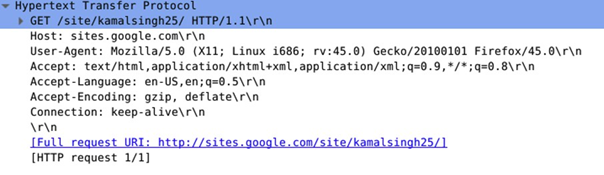
\includegraphics[width=1\columnwidth]{Pictures/GET.png}}
\lgf{\caption{Contenu d'une requête HTTP GET}}
\lge{\caption{Content of an HTTP GET request}}
\label{fig-GET}
\end{figure}

    \item  
        \lgf{\Index{HEAD} est utilisée pour récupérer uniquement les métadonnées présentes dans les en-têtes de réponse sans le corps de réponse ;}
        \lge{\Index{HEAD} est utilisée pour récupérer uniquement les métadonnées présentes dans les en-têtes de réponse sans le corps de réponse ;}
    \item  
        \lgf{\Index{POST} est utilisée pour indiquer au serveur une nouvelle ressource~;}
        \lge{\Index{POST} is used to inform the server of a new resource;}
    \item  
        \lgf{\Index{PUT} est utilisée pour stocker une ressource à l’endroit identifié par l’\ac{URI} dans la requête. Si la ressource existe déjà, elle sera modifiée~;}
        \lge{\Index{PUT} is used to store a resource at the location identified by the \ac{URI} in the request. If the resource already exists, it will be modified;}
    \item 
        \lgf{\Index{PATCH} permet au client de ne modifier qu’une partie de la ressource~;}
        \lge{\Index{PATCH} allows the client to modify only a part of the resource;}
    \item  
        \lgf{\Index{DELETE} est utilisée pour supprimer la ressource définie.}
        \lge{\Index{DELETE} is used to delete the specified resource.}
\end{itemize}

\Question{\lgf{Etat}\lge{State}}
{
\lgf{Le serveur garde un état des précédentes requêtes ?}
\lge{The server keeps track of previous requests?}
\begin{itemize}[label=$\circ$]
\item \Wrong{\Vrai}
\item \Correct{\Faux}
\end{itemize}
}
{
\lgf{Le serveur répond à une requête puis passe à la suivante. Il ne garde pas d'état. En revanche, une requête peut servir à modifier le contenu d'une ressource, et le resultat de la modification sera gardé.}
\lge{The server responds to one request and then moves on to the next. It does not keep any state. On the other hand, a request can be used to modify the content of a resource, and the result of the modification will be kept.}
}

\Question{Wold Wide Web}
{
\lgf{Le World Wide Web est basé sur ce principe des états pour~:}
\lge{The World Wide Web is based on this principle of states for:}
\begin{itemize}[label=$\circ$]
\item \Wrong{
    \lgf{fonctionner à la fois sur des ordinateurs et des téléphones portables,}
    \lge{work on both computers and smartphones,}
    }
\item \Correct{
    \lgf{pouvoir servir un grand nombre de requêtes,}
    \lge{be able to serve a large number of requests,}
    }
\item \Wrong{
    \lgf{chiffrer les communications.}
    \lge{encrypt communications.}
    }
\end{itemize}}
{
\lgf{Voir le commentaire précédent}
\lge{See previous comment}
}

\Question{\lgf{Repésentation de l'Information}\lge{Presentation of Information}}
{
\lgf{Quels sont les formats qui permettent de représenter des informations structurées (2 réponses)~: }
\lge{What formats are used to represent structured information (2 answers):}

  \begin{multicols}{4}
  \begin{itemize}[label=$\square$]
   \item \Wrong{Ethernet}
   \item \Wrong{IEEE}
   \item \Wrong{802.15.5}
   \item \Wrong{Wi-Fi}
   \item \Wrong{IPv4}
   \item \Wrong{IPv6}
   \item \Wrong{UDP}
   \item \Wrong{TCP}
   \item \Wrong{MQTT} 
   \item \Wrong{HTTP}
   \item \Wrong{CoAP}
   \item \Correct{XML}
   \item \Correct{JSON}
  \end{itemize}
  \end{multicols}
  }
  {Il s'agit de XML et JSON qui permettent d'envoyer des données stucturées. Les autres propositions indiquent des protocoles de transport de l'information de niveau 2, 3, 4 et 7.}
  
\Question{\lgf{Schéma}\lge{Scheme}}
{
\lgf{Dans l'URI \texttt{https://plido.net/unit/definition.html}, quel est le schéma ?}
\lge{In the URI \texttt{https://plido.net/unit/definition.html}, where is the scheme?}
\newline}
{\noindent
\lgf{\texttt{http}~: le Schéma indique comment sera construite l'URI.}
\lge{\texttt{http}~: the Scheme indicates how the URI will be constructed.}
}

\Question{\lgf{Authorité}\lge{Authority}}
{
\lgf{Dans l'URI \texttt{https://plido.net:8080/unit/definition.html}, quelle est l'autorité ?}
\lge{In the URI \texttt{https://plido.net:8080/unit/definition.html}, where is the authority?}
\newline}
{\noindent
\lgf{\texttt{plido.net:8080}~: il s'agit de la séquence globalement unique.}
\lge{\texttt{plido.net:8080}~: this is the globally unique sequence.}
}


\lgf{\section {Modèle Publish/Subscribe}}
\lge{\section {Publish/Subscribe Model}}

\lgf{Il existe d’autres formalismes que REST. Un autre formalisme, très populaire, est orienté "diffusion" en utilisant le principe ”publication/abonnement” ou ”\Index{publish/subscribe}”. Comme nous allons le montrer dans la suite, même si les fonctionnalités entre ces deux modes peuvent sembler similaires à HTTP, la philosophie de conception est très différente : publish/subscribe vise des applications intégrées tandis que REST vise l’interopérabilité globale. }
\lge{There are other formalisms than REST. Another formalism, very popular, is broascast oriented by using the "\Index{publish/subscribe}" principle. As we will show in the following, even if the functionalities between these two modes may seem similar to HTTP, the design philosophy is very different: publish/subscribe aims at integrated applications while REST aims at global interoperability. }

         \vspace{1em}


\lgf{Le modèle publish/subscribe fait le découplage entre l’expéditeur d’un message et son destinataire. Dans ce paradigme (cf. figure~\vref{fig-mqtt}), il existe des ”Publishers” qui produisent des données ou des messages et envoient le message à une entité généralement appelée ”Broker”. En outre, les messages peuvent être classés en ”Topics”, contenus ou types, etc. Ensuite, il existe des abonnés qui souscrivent au broker, par exemple à un topic donné, afin de recevoir les messages qui les intéressent, comme montré dans le schéma.}
\lge{The publish/subscribe model makes the decoupling between the sender of a message and its recipient. In this paradigm (see figure~\vref{fig-mqtt}), there are "Publishers" who produce data or messages and send the message to an entity generally called "Broker". In addition, messages can be classified into "Topics", contents or types, etc. Then, there are subscribers who subscribe to the broker, for example to a given topic, in order to receive the messages that interest them, as shown in the diagram.}

\begin{figure}
    \centering
    
    \begin{tikzpicture}
    
    \coordinate (brok) at (6, 4.5);
    \draw (brok) node (brokbox)[thick, rectangle, draw, minimum width=1cm, minimum height=6cm]{};
    \draw (brokbox.north) node [above]{Broker};    
    

    \coordinate (bat) at (-0.7,1.5);
    \coordinate (bate) at ([xshift=3cm]bat);
    
    \foreach \floor in {1,...,3} {
        \coordinate (init) at (0, \floor*2);
        \node[inner sep=0pt] (co2) at (init)
            {
\includegraphics[width=20pt]{Pictures/logo-co2.png}};
            
        \node[inner sep=0pt] (humi) at ([xshift=.3cm, yshift=0.3cm]co2.east)
            {
\includegraphics[width=15pt]{Pictures/logo-humi.png}};
        \node[inner sep=0pt] (press) at ([xshift=.3cm, yshift=0.3cm]humi.east)
            {
\includegraphics[width=17pt]{Pictures/logo-press.png}};           
        \node[inner sep=0pt] (temp) at ([xshift=.2cm, yshift=0.3cm]press.east)
            {
\includegraphics[width=10pt]{Pictures/logo-temp.png}};  
            
        \draw[->, dotted] (co2) -- node {\tiny{/sensor/bA/floor\floor/co2}} (brok|-co2);
        \draw[->, dotted] (humi) -- node {\tiny{/sensor/bA/floor\floor/humi}}(brok|-humi);
        \draw[->, dotted] (press) -- node {\tiny{/sensor/bA/floor\floor/pres}}(brok|-press);
        \draw[->, dotted] (temp) -- node {\tiny{/sensor/bA/floor\floor/temp}} (brok|-temp);
            
        \draw ([yshift=0.1cm]temp.north -| bat) coordinate(a) -- ([yshift=0.1cm]temp.north -| bate) coordinate(b);
        
        \draw ([yshift=-.5cm]a) node [left] {floor \floor};
    }
    

    \draw (bat) --node [below] {\lgf{bâtiment A}\lge{Building A}} (bate);
    \draw (bat) -- (a);
    \draw (bate) -- (b);
    
    \draw (11, 7) node (app1) [draw, cloud, minimum height=2cm, minimum width=3cm]{};
    \draw (app1) node [text width=3cm, text centered]{Floor 2\\monitoring\\};
    
    \draw [dashed, ->] (app1) -- node [sloped, above] {\tiny{sub /sensor/bA/floor2/*}} (brokbox.70); 

    \draw (10, 3) node (app2) [draw, cloud, minimum height=2cm, minimum width=3cm]{};
    \draw (app2) node [text width=3cm, text centered]{Temperature\\monitoring\\};
    
    \draw [dashed, ->] (app2) -- node [sloped, above] {\tiny{sub /sensor/bA/*/temp}} (brokbox.300); 
    \end{tikzpicture}
    
    \lgf{\caption{Exemple de topics MQTT.}}
    \lge{\caption{Example of MQTT topics.}}
    
    \label{fig-mqtt}
\end{figure}



\lgf{Le broker peut alors utiliser des filtres pour envoyer uniquement ces messages aux abonnés du topic concerné. Il existe plusieurs protocoles Publish-Subscribe tels que \acl{MQTT} (\acs{MQTT}), \acl{AMQP} (\acs{AMQP}), \acl{JMS} (\acs{JMS}) ou \acl{XMPP} (\acs{XMPP}).}
\lge{The broker can then use filters to send only these messages to the subscribers of the concerned topic. There are several Publish-Subscribe protocols such as \acl{MQTT} (\acs{MQTT}), \acl{AMQP} (\acs{AMQP}), \acl{JMS} (\acs{JMS}) or \acl{XMPP} (\acs{XMPP}).}

\subsection{MQTT}

\lgf{MQTT est détaillé dans la suite du cours car il est très populaire pour la communication entre processus, mais également dans l’internet des objets.}
\lge{MQTT is detailed in the rest of the course because it is very popular for communication between processes, but also in the Internet of Things.}

\lgf{Développé initialement par IBM en 1999, pour le middleware MQSeries, il est devenu une norme OASIS en 2013, puis en 2016 une norme ISO\footnote{\url{http://docs.oasis-open.org/mqtt/mqtt/v3.1.1/errata01/os/mqtt-v3.1.1-errata01-os-complete.pdf}}. }
\lge{Originally developed by IBM in 1999, for the MQSeries middleware, it became an OASIS standard in 2013, and in 2016 an ISO standard\footnote{\url{http://docs.oasis-open.org/mqtt/mqtt/v3.1.1/errata01/os/mqtt-v3.1.1-errata01-os-complete.pdf}}. }


\lgf{Imaginons par exemple que plusieurs capteurs soient installés, sur plusieurs étages, dans deux bâtiments A et B. Certains capteurs collectent des informations sur la température et d’autres collectent des informations sur l’humidité. Ces capteurs peuvent envoyer les données régulièrement à un broker central.}
\lge{For example, let's imagine that several sensors are installed, on several floors, in two buildings A and B. Some sensors collect temperature information and others collect humidity information. These sensors can send the data regularly to a central broker.}

\lgf{Les données peuvent être classées en différentes rubriques qui peuvent également être organisées de manière hiérarchique. Par exemple, le topic /sensor signifie "toutes les données de capteurs", \texttt{/sensor/buildingA/} signifie "des données de capteurs uniquement installées dans le bâtiment A". En plus, \texttt{/sensor/buildingA/floor3/temperature} pourrait signifier "des données de capteurs de température installés uniquement au troisième étage dans le bâtiment A".}
\lge{The data can be classified into different topics which can also be organized hierarchically. For example, the topic /sensor means "all sensor data", \texttt{/sensor/buildingA/} means "sensor data only installed in building A". In addition, \texttt{/sensor/buildingA/floor3/temperature} could mean "temperature sensor data installed only on the third floor in building A".}

\lgf{Certains abonnés peuvent s’abonner aux messages en fonction de leur intérêt. Ainsi, un abonné intéressé uniquement par les données d’humidité de l'ensemble du bâtiment B peut s’abonner au sujet \texttt{/sensor/buildingB /*/humidity} et le broker n’enverra que ces données à cet abonné.}
\lge{Some subscribers may subscribe to messages based on their interest. For example, a subscriber interested only in the humidity data of the whole building B can subscribe to the topic \texttt{/sensor/buildingB/*/humidity} and the broker will send only this data to this subscriber.}

\lgf{\subsection{différence avec REST}}
\lge{\subsection{difference with REST}}

\lgf{Les principaux avantages du paradigme publish-subscribe par rapport au paradigme client-serveur, tels qu'inclus en REST, sont les suivants~:}
\lge{The main advantages of the publish-subscribe paradigm over the client-server paradigm, as included in REST, are the following:}

\begin{itemize}
\item 
    \lgf{faible couplage entre émetteur et récepteur, le broker sert d'intermédiaire et stocke les informations ;}
    \lge{weak coupling between sender and receiver, the broker acts as an intermediary and stores the information;}
    
\item 
    \lgf{passage à l’échelle. Les données provenant d'une source ne sont émises qu'une fois par la source. Le broker les recopie vers tous les abonnés. Dans un mode client/serveur, les données doivent être émises par le serveur autant que fois que les clients le demandent.}
    \lge{scaling. Data from a source is sent out only once by the source. The broker copies it to all subscribers. In a client/server mode, the data must be sent by the server as many times as the clients request.}
\end{itemize}


\lgf{L’absence de couplage entre l’expéditeur et le destinataire se fait en termes d’espace, de temps et de synchronisation. Celui qui publie les données a une tâche simplifiée. Il n'a pas à gérer ou connaître ceux qui les consomment, il n'a qu’à les envoyer au broker.}
\lge{The lack of coupling between the sender and the receiver is done in terms of space, time and synchronization. The one who publishes the data has a simplified task. He doesn't have to manage or know who is consuming it, he only has to send it to the broker.}

\lgf{MQTT est très léger et conçu pour les périphériques de faibles puissances. Il a une très petite empreinte logicielle et est optimisé pour fonctionner dans les environnements à faible bande passante. Cela rend MQTT idéal pour les applications IoT. Malgré tout, l’usage de TCP et des très nombreux acquittements peut s’avérer lourds pour les équipements ou les réseaux très contraints. Une version plus légère basée sur UDP existe pour ces cas d’usage, mais elle est peu utilisée.}
\lge{MQTT is very lightweight and designed for low-power devices. It has a very small software footprint and is optimized to work in low-bandwidth environments. This makes MQTT ideal for IoT applications. Even so, the use of TCP and the many, many acknowledgements can be cumbersome for highly constrained devices or networks. A lighter version based on UDP exists for these use cases, but it is not widely used.}



\lgf{S'ils se ressemblent, les principes de nommage des topics MQTT et des URI REST sont complètement différents. Par rapport à MQTT, le chemin dans l'URI n'a pas de sémantique. Il a juste vocation à être unique. Il ne peut pas être utilisé pour agréger plusieurs sources d'information. Si deux capteurs publient respectivement sur les topics \texttt{/sensor/buildingA/temperature} et \texttt{/sensor/buildingB/temperature}, un subscriber peut s'abonner au topic \texttt{/sensor/*/temperature} pour recevoir toutes les mesures ; ce qui est impossible avec REST : il faudra autant de requêtes que de capteurs pour récupérer l'ensemble des mesures.}
\lge{Although they are similar, the naming principles of MQTT topics and REST URIs are completely different. Compared to MQTT, the path in the URI has no semantics. It is just meant to be unique. It cannot be used to aggregate multiple information sources. If two sensors publish respectively on the topics \texttt{/sensor/buildingA/temperature} and \texttt{/sensor/buildingB/temperature}, a subscriber can subscribe to the topic \texttt{/sensor/*/temperature} in order to receive all the measurements ; this is impossible with REST : it will be necessary to make as many requests as sensors to get all the measurements.}


\lgf{Les URI sont simplement uniques au monde par leur construction alors que les topics du MQTT sont spécifiques à une application. Un topic MQTT peut être interprété différemment par deux applications différentes. Cela ne permet pas une interopérabilité sémantique. Les abonnés doivent être construits avec une connaissance des topics utilisés par les publieurs.}
\lge{URIs are simply unique to the world in their construction, whereas MQTT topics are application specific. An MQTT topic can be interpreted differently by two different applications. This does not allow for semantic interoperability. Subscribers must be constructed with knowledge of the topics used by the publishers.}

